\section{Results}
  \label{sec:results}

Our experiments reveal that the choice of coverage criterion does have an impact
on the performance of test data generation. 
Figure~\ref{fig:crites} shows the results of the experiment for the BioSQL
schema, a real world schema used in biology created by the
Open Bioinformatics Foundation.
The graph shows how the choice of coverage criteria impacts
runtime as the size of the input schema increases. The following table shows
the worst-case time complexity of \textit{SchemaAnalyst} using the
chosen criterion.

\begin{figure*}
\centering
  \centering
  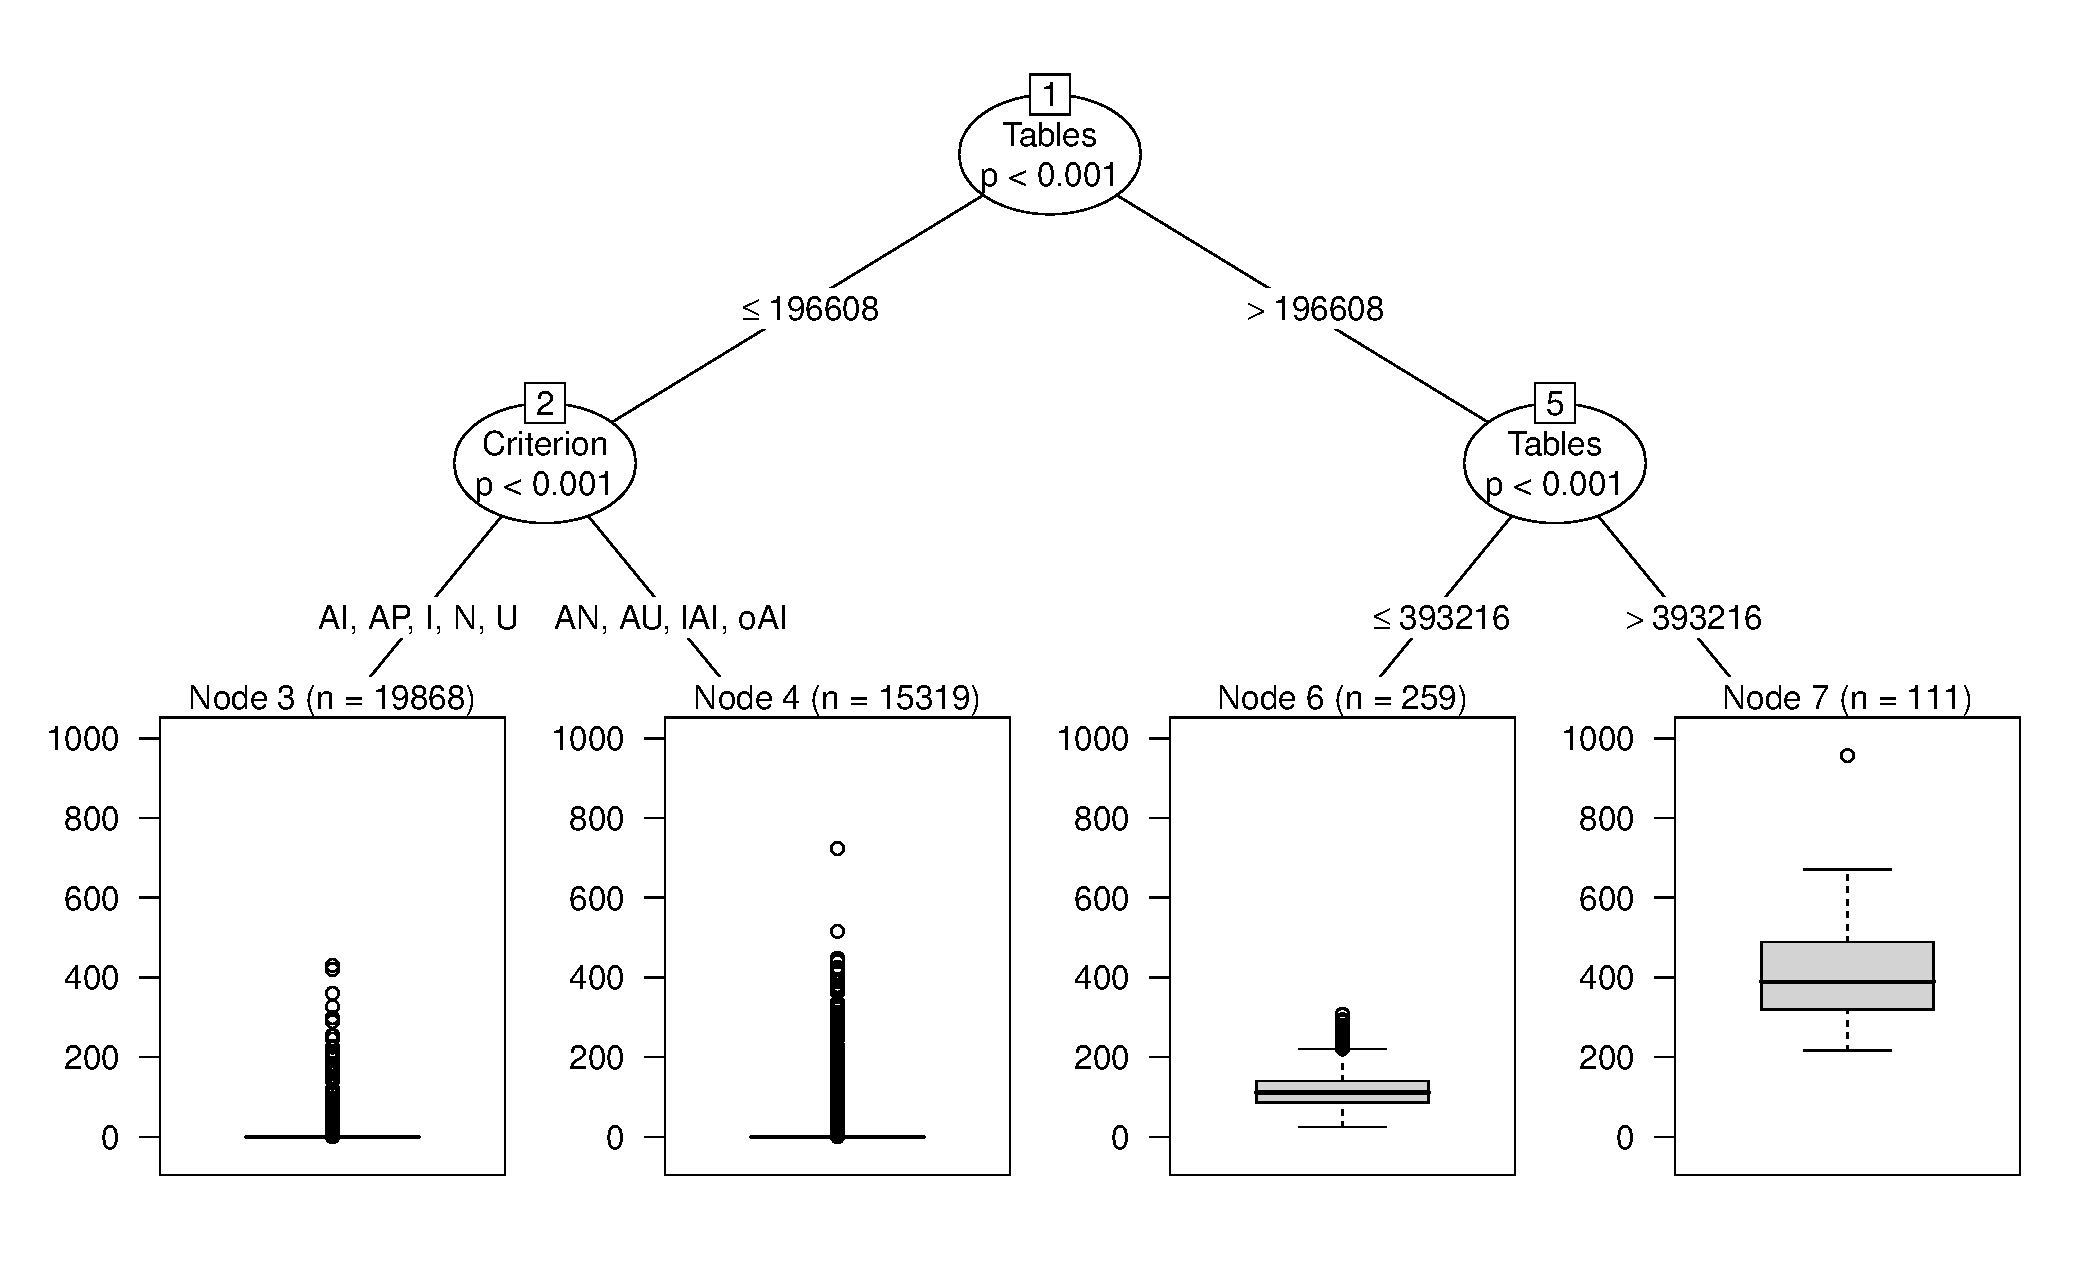
\includegraphics[width=.75\linewidth]{../diagrams/AllTree.pdf}
  \caption{Regression tree using all variables to predict runtime in
  minutes. \vspace{-.15in}}
  \label{fig:crites}
  \vspace{-.15in} 
\end{figure*}

\begin{figure*}
\centering
  \centering
  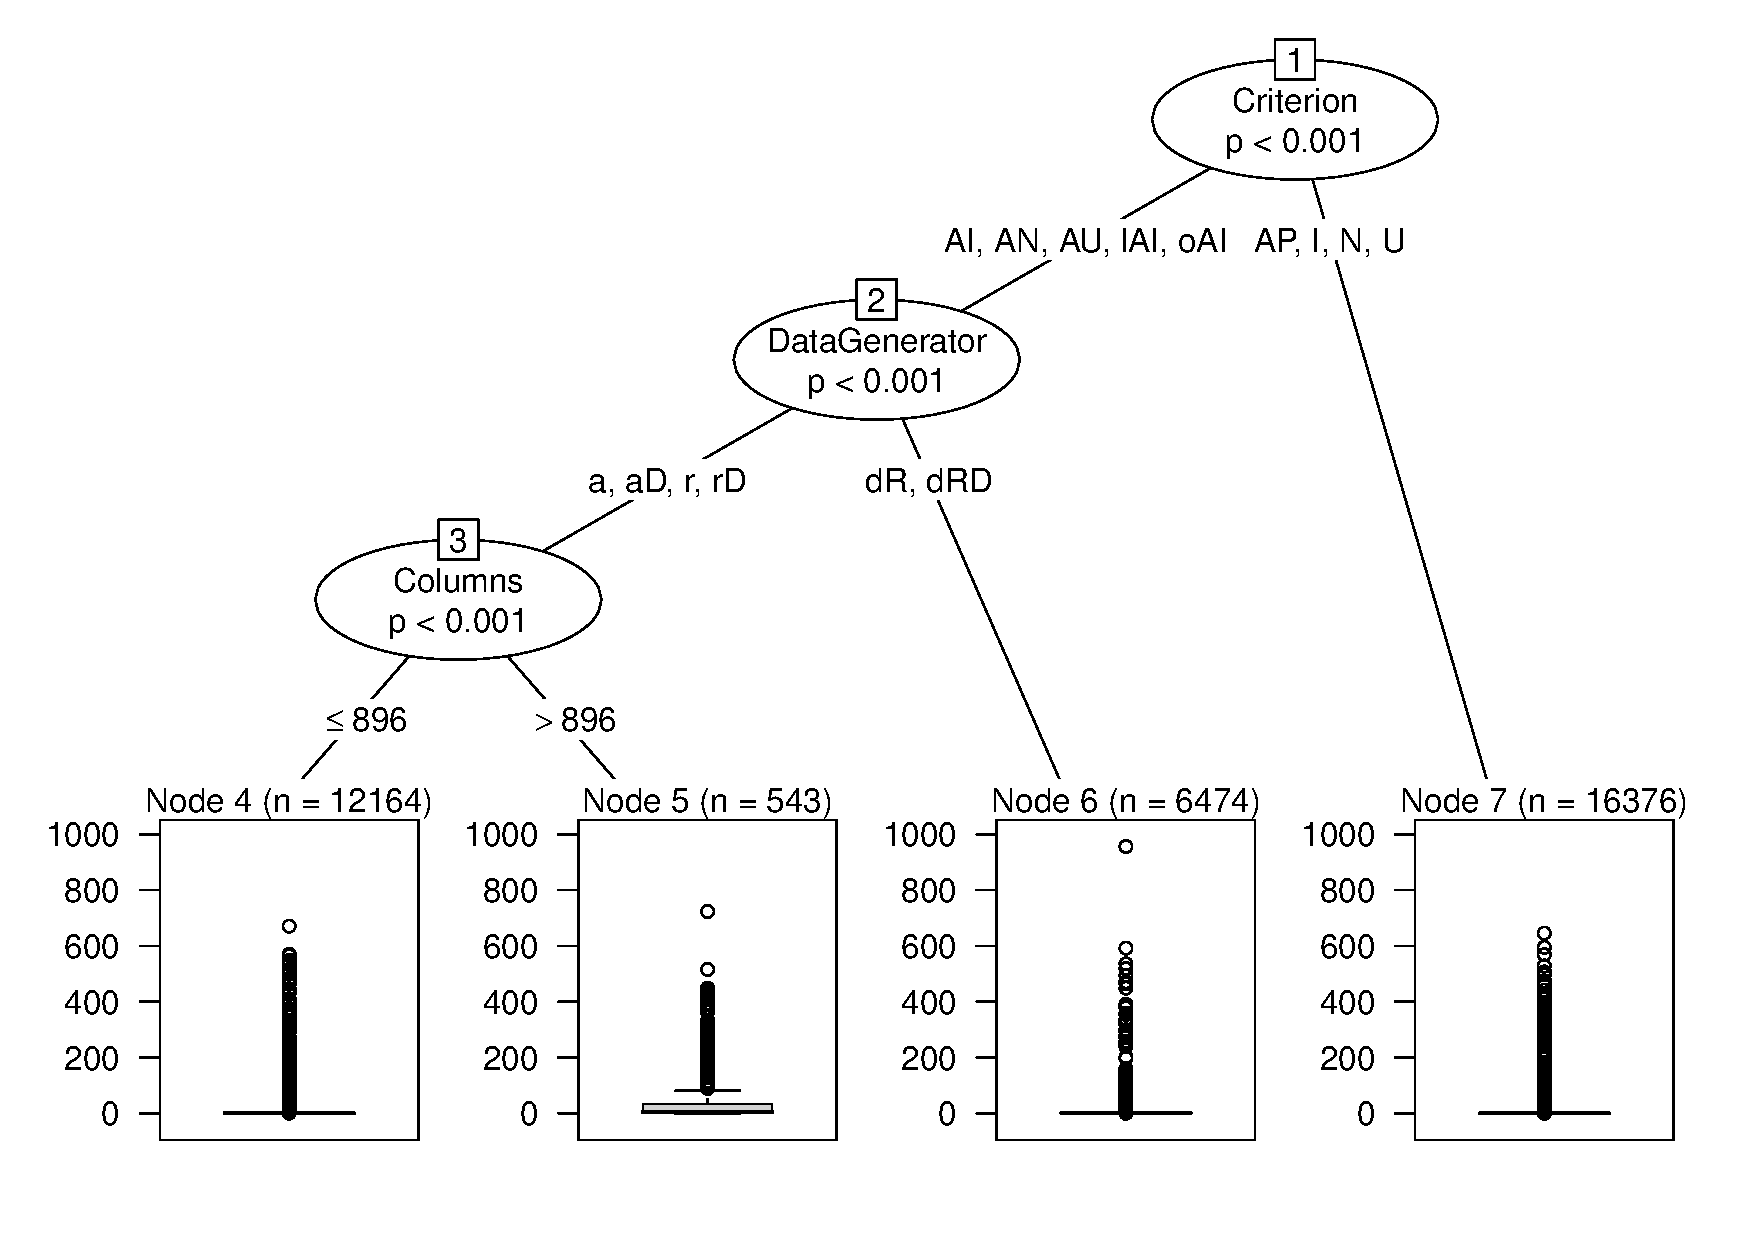
\includegraphics[width=.75\linewidth]{../diagrams/NoTableCtreesd.pdf}
  \caption{Regression tree predicting runtime excluding Tables.\vspace{-.15in}}
  \label{fig:crites}
  \vspace{-.15in} 
\end{figure*}


\begin{figure}
\centering
  \centering
  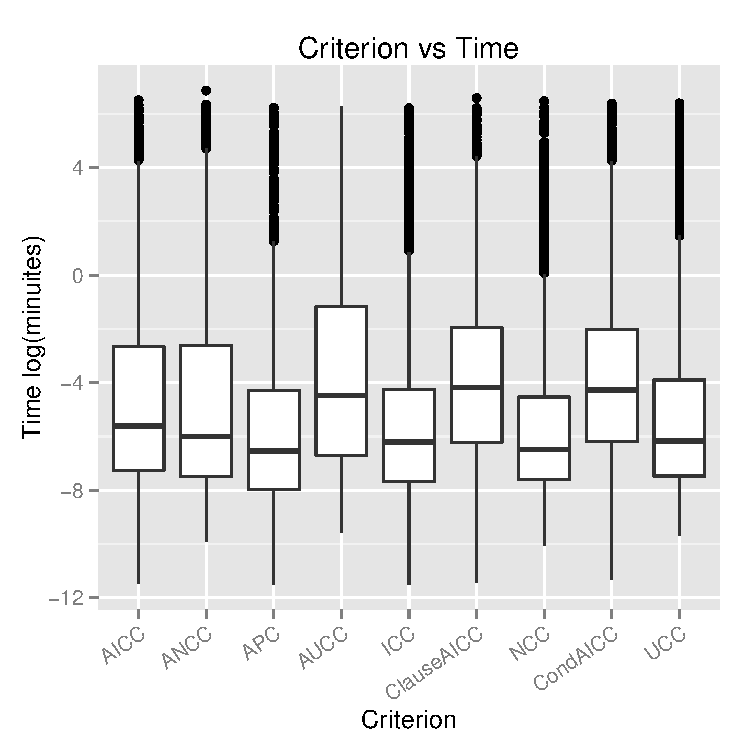
\includegraphics[width=1\linewidth]{../diagrams/CriterionvsTime.pdf}
  \caption{Coverage criterion versus runtime in minutes.\vspace{-.15in}}
  \label{fig:crites}
  \vspace{-.15in} 
\end{figure}

\begin{figure}
\centering
  \centering
  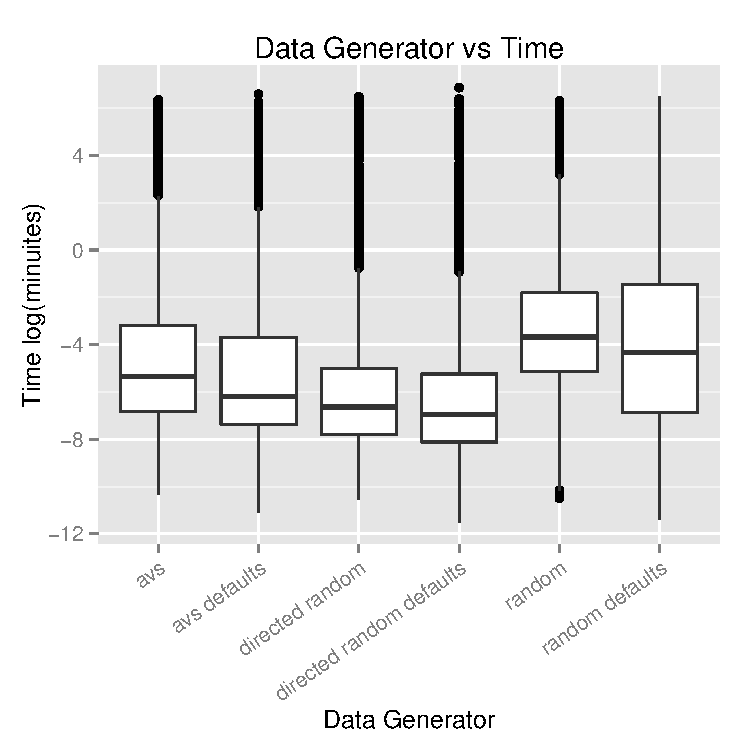
\includegraphics[width=1\linewidth]{../diagrams/DataGeneratorvsTime.pdf}
  \caption{Data generator versus runtime in minutes.\vspace{-.15in}}
  \label{fig:crites}
  \vspace{-.15in} 
\end{figure}


\begin{table}[h]
\begin{tabular}{ll|ll}
Criterion & Complexity & Criterion  & Complexity \\ \hline
ICC       & $O(n\log n)$ & UCC        & $O(n\log n)$ \\
AUCC      & $O(n)$       & ClauseAICC & $O(n)$       \\
CondAICC  & $O(n)$       & AICC       & $O(n)$       \\
ANCC      & $O(n\log n)$ & APC        & $O(n)$      
\end{tabular}
\end{table}

\begin{table*}[h]
\begin{tabular}{llllllllll}
           & APC      & ANCC     & CondAICC & NCC      & AUCC     & AICC     & ClauseAICC & ICC      & UCC   \\ 
APC        & NA       & 0.425    & 0.337    & 0.484    & 0.334    & 0.413    & 0.329      & 0.481    & 0.449 \\
ANCC       & 2.20E-16 & NA       & 0.407    & 0.561    & 0.405    & 0.484    & 0.399      & 0.554    & 0.526 \\
CondAICC   & 2.20E-16 & 2.20E-16 & NA       & 0.671    & 0.503    & 0.581    & 0.492      & 0.656    & 0.634 \\
NCC        & 1.20E-02 & 2.20E-16 & 2.20E-16 & NA       & 0.335    & 0.417    & 0.322      & 0.491    & 0.461 \\
AUCC       & 2.20E-16 & 2.20E-16 & 6.92E-01 & 2.20E-16 & NA       & 0.577    & 0.490      & 0.651    & 0.628 \\
AICC       & 2.20E-16 & 1.70E-02 & 2.20E-16 & 2.20E-16 & 2.20E-16 & NA       & 0.412      & 0.571    & 0.547 \\
ClauseAICC & 2.20E-16 & 2.20E-16 & 2.72E-01 & 2.20E-16 & 1.40E-01 & 2.20E-16 & NA         & 0.662    & 0.641 \\
ICC        & 4.00E-03 & 2.20E-16 & 2.20E-16 & 1.83E-01 & 2.20E-16 & 2.20E-16 & 2.20E-16   & NA       & 0.472 \\
UCC        & 9.30E-16 & 3.83E-05 & 2.20E-16 & 7.36E-10 & 2.20E-16 & 5.73E-13 & 2.20E-16   & 9.29E-06 & NA    \\ 
\end{tabular}
\caption{For each pair of coverage criterions, lower left shows Wilcox
Rank Sum Test, upper right shows $\hat{A}_{12}$.}
\end{table*}


\begin{table*}[h]
\begin{tabular}{lllllll}
                         & random   & random defaults & directed random & directed random defaults & avs      & avs defaults \\
random                   & NA       & 0.538           & 0.740           & 0.789                    & 0.627    & 0.680        \\
random defaults          & 6.59E-13 & NA              & 0.673           & 0.701                    & 0.564    & 0.617        \\
directed random          & 2.20E-16 & 2.20E-16        & NA              & 0.543                    & 0.360    & 0.435        \\
directed random defaults & 2.20E-16 & 2.20E-16        & 9.74E-16        & NA                       & 0.328    & 0.395        \\
avs                      & 2.20E-16 & 2.20E-16        & 2.20E-16        & 2.20E-16                 & NA       & 0.572        \\
avs defaults             & 2.20E-16 & 2.20E-16        & 2.20E-16        & 2.20E-16                 & 2.20E-16 & NA          
\end{tabular}
\caption{For each pair of Data Generators, lower left shows Wilcox Rank
Sum Test, upper right shows $\hat{A}_{12}$.}
\end{table*}

% \begin{table*}[h]
% \begin{tabular}{llllllllll}
%     & APC       & ANCC
%     & CondAICC                                                    &
%     NCC                                                     &
%     AUCC                                                     &
%     AICC                                                    &
%     ClauseAICC                                                    &
%     ICC                                                      &
%     UCC                                                      \\
% APC  & NA       & \begin{tabular}[c]{@{}l@{}}0.425\\ small\end{tabular} & \begin{tabular}[c]{@{}l@{}}0.337\\ medium\end{tabular} & \begin{tabular}[c]{@{}l@{}}0.484\\ none\end{tabular}  & \begin{tabular}[c]{@{}l@{}}0.334\\ medium\end{tabular} & \begin{tabular}[c]{@{}l@{}}0.413\\ small\end{tabular} & \begin{tabular}[c]{@{}l@{}}0.329\\ medium\end{tabular} & \begin{tabular}[c]{@{}l@{}}0.481\\ none\end{tabular}   & \begin{tabular}[c]{@{}l@{}}0.449\\ none\end{tabular}   \\
% ANCC  & 2.20E-16 & NA                                                    & \begin{tabular}[c]{@{}l@{}}0.407\\ small\end{tabular}  & \begin{tabular}[c]{@{}l@{}}0.561\\ small\end{tabular} & \begin{tabular}[c]{@{}l@{}}0.405\\ small\end{tabular}  & \begin{tabular}[c]{@{}l@{}}0.484\\ none\end{tabular}  & \begin{tabular}[c]{@{}l@{}}0.399\\ small\end{tabular}  & \begin{tabular}[c]{@{}l@{}}0.554\\ none\end{tabular}   & \begin{tabular}[c]{@{}l@{}}0.526\\ none\end{tabular}   \\
% CondAICC & 2.20E-16 & 2.20E-16                                              & NA                                                     & \begin{tabular}[c]{@{}l@{}}.671\\ medium\end{tabular} & \begin{tabular}[c]{@{}l@{}}0.503\\ none\end{tabular}   & \begin{tabular}[c]{@{}l@{}}0.581\\ small\end{tabular} & \begin{tabular}[c]{@{}l@{}}0.492\\ none\end{tabular}   & \begin{tabular}[c]{@{}l@{}}0.656\\ medium\end{tabular} & \begin{tabular}[c]{@{}l@{}}0.634\\ small\end{tabular}  \\
% NCC   & 0.012    & 2.20E-16                                              & 2.20E-16                                               & NA                                                    & \begin{tabular}[c]{@{}l@{}}0.335\\ medium\end{tabular} & \begin{tabular}[c]{@{}l@{}}0.417\\ small\end{tabular} & \begin{tabular}[c]{@{}l@{}}0.322\\ medium\end{tabular} & \begin{tabular}[c]{@{}l@{}}0.491\\ none\end{tabular}   & \begin{tabular}[c]{@{}l@{}}0.461\\ none\end{tabular}   \\
% AUCC  & 2.20E-16 & 2.20E-16                                              & 0.692                                                  & 2.20E-16                                              & NA                                                     & \begin{tabular}[c]{@{}l@{}}0.577\\ small\end{tabular} & \begin{tabular}[c]{@{}l@{}}0.490\\ none\end{tabular}   & \begin{tabular}[c]{@{}l@{}}0.651\\ medium\end{tabular} & \begin{tabular}[c]{@{}l@{}}0.628\\ small\end{tabular}  \\
% AICC  & 2.20E-16 & 0.017                                                 & 2.20E-16                                               & 2.20E-16                                              & 2.20E-16                                               & NA                                                    & \begin{tabular}[c]{@{}l@{}}0.412\\ small\end{tabular}  & \begin{tabular}[c]{@{}l@{}}0.571\\ small\end{tabular}  & \begin{tabular}[c]{@{}l@{}}0.547\\ none\end{tabular}   \\
% ClauseAICC & 2.20E-16 & 2.20E-16                                              & 0.272                                                  & 2.20E-16                                              & 0.14                                                   & 2.20E-16                                              & NA                                                     & \begin{tabular}[c]{@{}l@{}}0.662\\ medium\end{tabular} & \begin{tabular}[c]{@{}l@{}}0.641\\ medium\end{tabular} \\
% ICC   & 0.004    & 2.20E-16                                              & 2.20E-16                                               & 0.1833                                                & 2.20E-16                                               & 2.20E-16                                              & 2.20E-16                                               & NA                                                     & \begin{tabular}[c]{@{}l@{}}0.472\\ none\end{tabular}   \\
% UCC   & 9.30E-16 & 3.83E-5                                               & 2.20E-16                                               & 7.36E-10                                              & 2.20E-16                                               & 5.73E-13                                              & 2.20E-16                                               & 9.29E-6                                                & NA                                                    
% \end{tabular}
% \caption{For each pair of Criterions, lower left shows Wilcox Rank Sum
% Test, upper right shows $\hat{A}_{12}$.}
% \end{table*}
%
% \begin{table*}[h]
% \begin{tabular}{lllllll}
%                          & random    & random defaults                                     & directed random                                       & \begin{tabular}[c]{@{}l@{}}directed random\\ defaults\end{tabular} & avs                                                   & avs defaults                                          \\
% random                   & NA        & \begin{tabular}[c]{@{}l@{}}.538\\ none\end{tabular} & \begin{tabular}[c]{@{}l@{}}.740\\ large\end{tabular}  & \begin{tabular}[c]{@{}l@{}}.789\\ large\end{tabular}               & \begin{tabular}[c]{@{}l@{}}.627\\ small\end{tabular}  & \begin{tabular}[c]{@{}l@{}}.680\\ meduim\end{tabular} \\
% random defaults          & 6.594e-13 & NA                                                  & \begin{tabular}[c]{@{}l@{}}.673\\ medium\end{tabular} & \begin{tabular}[c]{@{}l@{}}.701\\ medium\end{tabular}              & \begin{tabular}[c]{@{}l@{}}.564\\ small\end{tabular}  & \begin{tabular}[c]{@{}l@{}}.617\\ small\end{tabular}  \\
% directed random          & 2.2e-16   & 2.2e-16                                             & NA                                                    & \begin{tabular}[c]{@{}l@{}}.543\\ none\end{tabular}                & \begin{tabular}[c]{@{}l@{}}.360\\ small\end{tabular}  & \begin{tabular}[c]{@{}l@{}}.435\\ small\end{tabular}  \\
% directed random defaults & 2.2e-16   & 2.2e-16                                             & 9.735e-16                                             & NA                                                                 & \begin{tabular}[c]{@{}l@{}}.328\\ medium\end{tabular} & \begin{tabular}[c]{@{}l@{}}.395\\ small\end{tabular}  \\
% avs                      & 2.2e-16   & 2.2e-16                                             & 2.2e-16                                               & 2.2e-16                                                            & NA                                                    & \begin{tabular}[c]{@{}l@{}}.572\\ small\end{tabular}  \\
% avs defaults             & 2.2e-16   & 2.2e-16                                             & 2.2e-16                                               & 2.2e-16                                                            & 2.2e-16                                               & NA                                                   
% \end{tabular}
% \caption{For each pair of Data Genenerators, lower left shows Wilcox Rank Sum
% Test, upper right shows $\hat{A}_{12}$.}
% \end{table*}

Although ICC, UCC, and ANCC have worse scalability according to the
table ($O(n)$ vs $O(n\log n)$), the difference is not apparent for
realistically sized schemas, which are not likely to
be larger than 100 times the size of BioSQL, which contains 28 tables.
Therefore, we can conclude that ANCC is the most efficient criterion.  

As new data arrives, we hope to learn about the impact of other
parameters, and support our findings with additional schemas. 
Future work includes comparing the performance cost of these
parameters to their testing effectiveness, and the optimization of test data generation.
\subsection*{Threats to Validity}

Our technique for doubling the number of check constraints on the schema
is simply to duplicate the existing check constraints. It is possible
that \textit{SchemaAnalyst} does less work processing these copied check
constraints than it would given unique check constraints. However,
doubling the check constraints in this way is an easy to implement,
semantically significant way of evaluating \textit{SchemaAnalyst}.

Additionally, since worst-case time is only apparent for large $n$, 
it is possible that the experiment terminated too quickly.  To guard 
against this problem, Algorithms~\ref{alg:convergence} and~\ref{alg:tuning}
were tested on various other algorithms with known worst-case complexities, and 
found to be reliable.
